\documentclass[oneside,a4paper,14pt]{extarticle}
\usepackage[T2A]{fontenc} 
\usepackage[top=20mm,bottom=20mm,left=30mm,right=15mm]{geometry}

\usepackage[utf8]{inputenc}
\usepackage[russian]{babel}
\usepackage{microtype} % Улучшает переносы
\usepackage{textcomp}
\usepackage{indentfirst}
\usepackage{graphicx}
\usepackage{wrapfig}
\usepackage{caption}
\usepackage{amsmath}
\usepackage{amsfonts}
\usepackage{amsthm}
\usepackage[all]{xy}
\usepackage[breaklinks]{hyperref}
\usepackage{titlesec} 
\usepackage{listings}
\usepackage{booktabs}
\usepackage{array}
\usepackage{multirow}

\hyphenation{Logis-tic-Re-gres-sion Stan-dard-Sca-ler most-fre-quent}

\titleformat{\section}{\normalsize\bfseries}{\thesection}{1em}{} 
\titleformat{\subsection}{\normalsize\bfseries}{\thesubsection}{1em}{} 
\titleformat{\subsubsection}{\normalsize\bfseries}{\thesubsubsection}{1em}{} 

\renewcommand\baselinestretch{1.33}\normalsize
\setlength{\parindent}{1.25cm}

\begin{document}

\newpage\thispagestyle{empty}
\begin{center}
	МИНИСТЕРСТВО НАУКИ И ВЫСШЕГО ОБРАЗОВАНИЯ\\
	РОССИЙСКОЙ ФЕДЕРАЦИИ\\
	ФЕДЕРАЛЬНОЕ ГОСУДАРСТВЕННОЕ БЮДЖЕТНОЕ\\
	ОБРАЗОВАТЕЛЬНОЕ УЧРЕЖДЕНИЕ ВЫСШЕГО ОБРАЗОВАНИЯ\\
	<<ВЯТСКИЙ ГОСУДАРСТВЕННЫЙ УНИВЕРСИТЕТ>>\\
	Институт математики и информационных систем\\
	Факультет автоматики и вычислительной техники\\
	Кафедра электронных вычислительных машин
\end{center}
\vspace{30mm}

\begin{center}
	Отчёт по лабораторной работе №1\\
	по дисциплине\\
	<<Машинное обучение>>\\
	<<Полный цикл решения задачи классификации.>>\\
	<<Линейные модели и стохастический градиент.>>\\
\end{center}
\vspace{40mm}

\noindent
\begin{tabular}{l r}
	Выполнил студент гр. ИВТб-2303-06-00 \hspace{10mm} \rule[-1mm]{20mm}{0.15mm}\,/Перевозчиков Д.А./ \\ \\
	Проверил \hspace{65mm} \rule[-1mm]{20mm}{0.15mm}\,/Пащенко Д. Э./
\end{tabular}

\vfill
\begin{center}
	Киров\\
	2026
\end{center}

\newpage

\section{Цель работы}
Изучить начальные способы решения задачи многоклассовой классификации, процесс предобработки данных перед обучением моделей. Самостоятельно реализовать алгоритм стохастического градиентного спуска (SGD), исследовать влияние темпа обучения и L2-регуляризации, научиться подбирать гиперпараметры библиотечных моделей и оценивать качество их предсказаний.

\section{Вариант и данные}
\textbf{Особенности набора:} Все 64 признака являются  числовыми (коэффициенты Кархунена-Лоэва, описывающие форму объектов). Пропуски отсутствуют. Датасет сбалансирован (ровно 200 объектов на каждый из 10 классов), поэтому применять методы борьбы с дисбалансом не требуется, однако macro-усреднение метрик для объективной оценки приходится применить.


\begin{table}[h!]
  \centering
  \label{tab:protocol}
  \begin{tabular}{|l|p{9cm}|}
    \hline
    \textbf{Параметр} & \textbf{Значение} \\
    \hline
    RANDOM\_STATE & 1004 \\
    \hline
    Разбиение & \texttt{test\_size=0.2}, \texttt{stratify=y}, 
                 1600 объектов в Train и 400 в Test \\
    \hline
    Кросс-валидация & \texttt{StratifiedKFold(n\_splits=5, shuffle=True)} \\
    \hline
    Основная метрика & \texttt{macro-F1} (так как классов 10, и они равнозначны) \\
    \hline
    Правила preprocessing & Так как пропусков нет, импутация данных 
                             не требуется. Все числовые признаки масштабируются 
                             с помощью \texttt{StandardScaler} для корректной 
                             работы градиентного спуска \\
    \hline
  \end{tabular}
   \caption{Параметры экспериментального протокола} 
\end{table}


\newpage
\section{Ход работы и результаты}

\subsection{Baseline}
\textbf{CV-метрики baseline:} Accuracy = 0.1000, macro-F1 = 0.0182. 

Поскольку в датасете 10 классов и они идеально сбалансированы, стратегия \texttt{most\_frequent} просто угадывает один класс для всех объектов. Точность 10\% и крайне низкий F1 подтверждают, что датасет не имеет тривиального доминирующего класса. Любая содержательная модель должна значительно превзойти эти значения, чтобы доказать, что она использует признаки, а не случайное угадывание.

\subsection{SGD с нуля}
В нашей реализации параметр \textbf{$\tau$} отвечает за силу L2-регуляризации (штраф за рост весов). Параметр \textbf{$\eta$} -- это темп обучения (learning rate).

Изучая таблицу зависимости качества от $\eta$ (при фиксированном $\tau=10^{-4}$), мы можем заметить, что при увеличении шага обучения с 0.0001 до 0.1000 финальное значение функции потерь у обучающей выборки падает с 0.2153 до 0.0048, что говорит о сходимости модели. Однако функция потерь у валидационной выборки ведет себя нелинейно, при $\eta=0.0001$ значение функции = 0.2088 (модель не успевает сойтись), при $\eta=0.01$ значение  снижается до 0.0197, а при $\eta=0.1$ функция достигает минимума 0.0161, но норма весов при этом вырастает до 8.7914. Из этого делаем вывод, что слишком большой шаг обучения приводит к росту нормы весов и риску переобучения. Оптимальным значением является $\eta=0.01$.

\begin{figure}[ht]
    \centering
    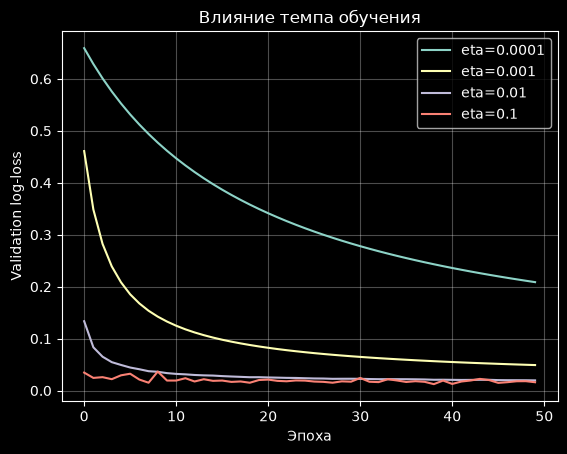
\includegraphics[width=0.75\textwidth]{images/g1.png}
    \caption{Влияние темпа обучения $\eta$ на validation loss}
\end{figure}

\begin{table}[ht]
\centering

\begin{tabular}{cccc}
\toprule
$\eta$ & final\_train\_loss & final\_val\_loss & weight\_norm \\
\midrule
0.0001 & 0.2153 & 0.2088 & 0.7944 \\
0.0010 & 0.0511 & 0.0491 & 2.2124 \\
0.0100 & 0.0149 & 0.0197 & 4.4856 \\
0.1000 & 0.0048 & 0.0161 & 8.7914 \\
\bottomrule
\end{tabular}
\caption{Влияние темпа обучения $\eta$ на качество модели}
\end{table} 
\newpage

\textbf{Влияние $\tau$} (при фиксированном $\eta=0.01$): Изучая таблицу зависимости качества от $\tau$, мы можем заметить, что при увеличении коэффициента регуляризации $\tau$ с 0.0000 до 0.0100 норма весов (\texttt{weight\_norm}) существенно снижается с 9.8225 до 2.7894. Это подтверждает теорию: L2-регуляризация <<сжимает>> веса, не давая модели переобучаться. При этом \texttt{val\_loss} растет с 0.0154 до 0.0491, так как модель становится более простой и жесткой, но это необходимая плата за обобщающую способность.

\begin{table}[ht]
\centering

\begin{tabular}{cccc}
\toprule
№ & $\tau$ & val\_loss & weight\_norm \\
\midrule
0 & 0.0000 & 0.0154 & 9.8225 \\
1 & 0.0001 & 0.0161 & 8.7914 \\
2 & 0.0100 & 0.0491 & 2.7894 \\
\bottomrule
\end{tabular}
\caption{Влияние коэффициента регуляризации $\tau$ на качество модели}
\end{table}

\begin{figure}[ht]
    \centering
    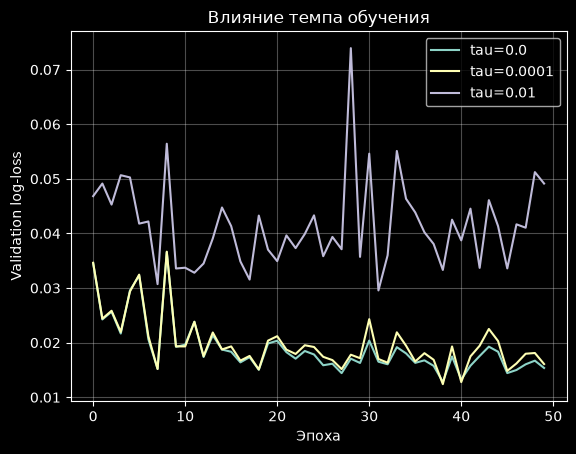
\includegraphics[width=0.75\textwidth]{images/g2.png}
    \caption{Влияние коэффициента регуляризации $\tau$ на качество модели}
\end{figure}


\newpage
\subsection{Библиотечные модели}
Для решения задачи был собран \texttt{Pipeline}, включающий \texttt{StandardScaler} и линейные классификаторы. Подбор гиперпараметров осуществлялся через \texttt{GridSearchCV} на кросс-валидации.

\begin{itemize}
    \item \textbf{SGDClassifier:} Подбирались \texttt{eta0} (темп обучения) и \texttt{alpha} (регуляризация). Лучший результат CV macro-F1 = 0.9449 достигнут при \texttt{eta0 = 0.01}, \texttt{alpha = 0.01}.
    \item \textbf{LogisticRegression:} Подбирался параметр \texttt{C} (обратная сила регуляризации). Лучший результат CV macro-F1 = 0.9443 при \texttt{C = 0.1}. 
\end{itemize}
Обе модели показали близкие результаты на кросс-валидации, что говорит о стабильности линейного разделения пространства признаков.

\begin{table}[ht]
\centering
\begin{tabular}{ccc}
\toprule
№ & Модель & Лучшие параметры \\
\midrule
1 & SGDClassifier & \texttt{alpha=0.01, eta0=0.01} \\
2 & LogisticRegression & \texttt{C=0.1} \\
0 & DummyClassifier & \texttt{strategy=most\_frequent} \\
\bottomrule
\end{tabular}
\caption{Сравнение моделей на кросс-валидации}

\end{table}

\newpage

\subsection{Финальный test}
На отложенной тестовой выборке \texttt{LogisticRegression} показала лучший результат (Accuracy = 0.9675, macro-F1 = 0.9675), чем \texttt{SGDClassifier} (Accuracy = 0.9600, macro-F1 = 0.9598). Обе модели значительно превзошли baseline.

\begin{table}[ht]
\centering
\begin{tabular}{cccccc}
\toprule
№ & Модель & Accuracy & Precision & Recall & F1-macro \\
\midrule
0 & DummyClassifier & 0.1000 & 0.010 & 0.1000 & 0.0182 \\
1 & SGDClassifier & 0.9600 & 0.961 & 0.9600 & 0.9598 \\
2 & LogisticRegression & 0.9675 & 0.969 & 0.9675 & 0.9675 \\
\bottomrule
\end{tabular}
\caption{Результаты на тестовой выборке}

\end{table}

\begin{table}[ht]
\centering
\begin{tabular}{lccccc}
\toprule
Класс & Precision & Recall & F1-score & Support \\
\midrule
1 & 0.95 & 1.00 & 0.98 & 40 \\
2 & 0.93 & 1.00 & 0.96 & 40 \\
3 & 1.00 & 1.00 & 1.00 & 40 \\
4 & 0.94 & 0.85 & 0.89 & 40 \\
5 & 1.00 & 0.95 & 0.97 & 40 \\
6 & 0.97 & 0.95 & 0.96 & 40 \\
7 & 0.97 & 0.97 & 0.97 & 40 \\
8 & 0.91 & 0.97 & 0.94 & 40 \\
9 & 1.00 & 0.95 & 0.97 & 40 \\
10 & 0.93 & 0.95 & 0.94 & 40 \\
\midrule
\textbf{Accuracy} & \multicolumn{3}{c}{0.96} & 400 \\
\textbf{Macro avg} & 0.96 & 0.96 & 0.96 & 400 \\
\textbf{Weighted avg} & 0.96 & 0.96 & 0.96 & 400 \\
\bottomrule
\end{tabular}
\caption{Отчет о классификации (LogisticRegression)}

\end{table}

\begin{figure}[ht]
    \centering
    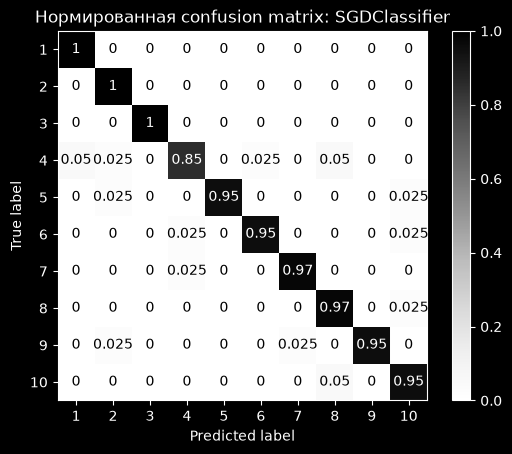
\includegraphics[width=0.7\textwidth]{images/m1.png}
    \caption{Матрица ошибок (Confusion Matrix) для LogisticRegression}
\end{figure}

\newpage
\subsection{Анализ ошибок}
Анализ таблицы наиболее уверенных ошибок показывает, что модель чаще всего ошибается на объектах классов \textbf{4, 5, 6, 8 и 10}. Наиболее характерные ошибки:
\begin{itemize}
    \item Класс 4 путается с 8 (объект 602, confidence~$= 0.68$) и с 2 (объект 649, confidence~$= 0.65$).
    \item Класс 5 ошибочно классифицируется как 10 (объект 882, confidence~$= 0.66$).
    \item Класс 8 путается с 10 (объект 1444, confidence~$= 0.52$).
    \item Класс 4 путается с 1 (объект 792, confidence~$= 0.51$).
    \item Класс 5 ошибочно предсказывается как 2 (объект 960, confidence~$= 0.49$).
    \item Класс 6 путается с 4 (объект 1092, confidence~$= 0.48$) и с 10 (объект 1069, confidence~$= 0.47$).
    \item Класс 10 путается с 8 (объект 1939, confidence~$= 0.47$).
\end{itemize}

\textbf{Интерпретация причин ошибок:}
\begin{enumerate}
    \item \textbf{Линейная неразделимость:} Датасет \texttt{mfeat-karhunen} описывает формы объектов через коэффициенты Кархунена. Некоторые цифры похожи друг на друга и выдают близкие значения в пространстве признаков по некоторым соседним признакам.
    \item \textbf{Пересечение классов:} Объекты классов 6 и 10, а также 4 и 8 имеют близкие значения признаков (например, по \texttt{att1}, \texttt{att2}), из-за чего модель выдает высокую уверенность, но ошибается в выборе.
    \item \textbf{Шум в данных:} Некоторые объекты имеют аномальные значения признаков, что смещает линейную оценку.
\end{enumerate}

\begin{table}[ht]
\centering
\begin{tabular}{cccccccc}
\toprule
Idx & att1 & att2 & att4 & att7 & true & pred & conf \\
\midrule
602 & 14.22 & 5.82 & 2.30 & -1.67 & 4 & 8 & 0.68 \\
882 & -3.18 & -5.16 & 7.90 & -3.14 & 5 & 10 & 0.65 \\
649 & 5.36 & 5.73 & 9.23 & -1.70 & 4 & 2 & 0.65 \\
652 & -2.07 & -1.71 & 10.75 & -0.59 & 4 & 8 & 0.57 \\
1444 & 4.67 & -7.92 & 3.44 & 0.65 & 8 & 10 & 0.52 \\
792 & -5.48 & -1.55 & 8.86 & -8.87 & 4 & 1 & 0.51 \\
960 & -0.18 & 7.61 & 4.62 & 1.04 & 5 & 2 & 0.48 \\
1092 & -9.08 & -3.57 & 6.25 & -3.71 & 6 & 4 & 0.47 \\
1939 & 13.38 & -0.24 & -4.63 & -3.68 & 10 & 8 & 0.47 \\
1069 & -0.78 & -1.67 & -2.13 & -5.11 & 6 & 10 & 0.47 \\
\bottomrule
\end{tabular}
\caption{Примеры наиболее уверенных ошибок классификации (ключевые признаки)}

\end{table}

\subsection{Анализ коэффициентов}
Анализ коэффициентов модели \texttt{LogisticRegression} для класса 1 показывает, что наиболее важными признаками являются \texttt{att1} (коэффициент -1.007), \texttt{att7} (-0.934), \texttt{att2} (-0.907), \texttt{att4} (-0.472) и \texttt{att20} (0.450). Эти признаки вносят наибольший вклад в разделение класса 1 от остальных. Отрицательные коэффициенты означают, что увеличение значения признака снижает вероятность принадлежности к классу 1.

\begin{table}[ht]
\centering
\begin{tabular}{ccc}
\toprule
№ & Признак & |Коэффициент| \\
\midrule
0 & \texttt{num\_\_att1} & 1.006667 \\
6 & \texttt{num\_\_att7} & 0.934140 \\
1 & \texttt{num\_\_att2} & 0.907004 \\
3 & \texttt{num\_\_att4} & 0.471681 \\
19 & \texttt{num\_\_att20} & 0.450484 \\
9 & \texttt{num\_\_att10} & 0.442513 \\
4 & \texttt{num\_\_att5} & 0.436300 \\
13 & \texttt{num\_\_att14} & 0.428139 \\
25 & \texttt{num\_\_att26} & 0.422736 \\
18 & \texttt{num\_\_att19} & 0.420888 \\
22 & \texttt{num\_\_att23} & 0.377420 \\
21 & \texttt{num\_\_att22} & 0.368085 \\
5 & \texttt{num\_\_att6} & 0.355352 \\
10 & \texttt{num\_\_att11} & 0.334465 \\
8 & \texttt{num\_\_att9} & 0.296371 \\
\bottomrule
\end{tabular}
\caption{Топ-15 наиболее важных признаков для класса 1}

\end{table}

\newpage
\section*{Выводы}
\begin{enumerate}
    \item Базовая модель (\texttt{DummyClassifier}) подтвердила, что обычное угадывание на сбалансированном 10-классовом датасете дает macro-F1 всего 0.0182. Это даёт нам нижнюю границу для оценки качества более "умных" моделей.
    \item При ручной реализации SGD было выявлено, что увеличение шага обучения $\eta$ сверх меры (0.1) приводит к росту нормы весов до 8.7914: значение функции потерь на обучающей выборке падает до 0.0048, на валидационной достигает 0.0161. Оптимальным балансом между сходимостью и устойчивостью оказалось $\eta=0.01$.
    \item Увеличение коэффициента L2-регуляризации $\tau$ с 0 до 0.01 привело к снижению нормы весов с 9.8225 до 2.7894, что показывает работу штрафа за сложность модели.
    \item Усвоены принципы построения \texttt{Pipeline} и  разделения Train/Test/CV.
    \item Сравнение библиотечных моделей показало, что \texttt{LogisticRegression} (F1=0.9675 на test) работает немного стабильнее, чем \texttt{SGDClassifier} (F1=0.9598), хотя на CV они показали близкие результаты (0.9443 и 0.9449 соответственно).


\end{enumerate}

\newpage


\end{document}